\documentclass{ximera}
\title{Quadratic Functions and Applications}

\outcome{Find the vertex of a quadratic function using the vertex formula.}
\outcome{Write a quadratic function in vertex form by completing the square.}
\outcome{Identify key features of a parabola: vertex, intercepts, axis of symmetry, domain, range.}
\outcome{Construct a quadratic function from given conditions.}
\outcome{Solve applied maximum/minimum problems using quadratic functions.}

\begin{document}
\begin{abstract}
\end{abstract}
\maketitle

\textbf{Learning Objectives:}
\begin{itemize}
  \item Find the vertex of a quadratic function using the vertex formula.
  \item Write a quadratic function in vertex form by completing the square.
  \item Identify key features of a parabola: vertex, intercepts, axis of symmetry, domain, range.
  \item Construct a quadratic function from given conditions.
  \item Solve applied maximum/minimum problems using quadratic functions.
\end{itemize}
\medskip

\section*{Quick Check}

\begin{problem}
A ball is tossed into the air from ground level. Its height in feet after $t$ seconds is $h(t) = -16t^2 + 64t$. At what time does the ball reach its maximum height?
\begin{hint}
The maximum of a quadratic $at^2+bt$ occurs at $t = -\dfrac{b}{2a}$.
\end{hint}
\begin{multipleChoice}
  \choice{1 second}
  \choice[correct]{2 seconds}
  \choice{3 seconds}
  \choice{4 seconds}
\end{multipleChoice}
\end{problem}

\begin{problem}
The graph of a quadratic function is shown below.

\begin{center}
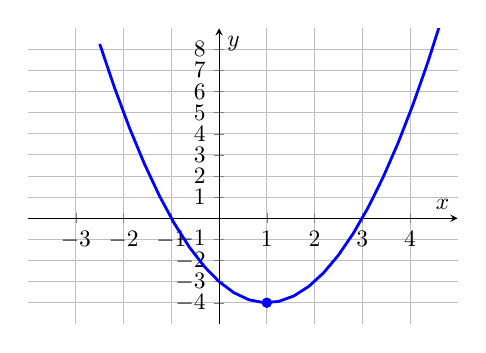
\begin{tikzpicture}[scale=0.85]
\begin{axis}[
  axis lines=middle,
  xmin=-4, xmax=5,
  ymin=-5, ymax=9,
  xtick={-3,...,4},
  ytick={-4,...,8},
  grid=major,
  width=8cm, height=6cm,
  xlabel={$x$}, ylabel={$y$}
]
\addplot[very thick, blue, domain=-2.5:5] {(x-1)^2 - 4};
\addplot[only marks, mark=*, blue] coordinates {(1,-4)};
\end{axis}
\end{tikzpicture}
\end{center}

Which equation could represent this graph?
\begin{hint}
Identify the vertex from the graph and check which equation has that vertex in the form $y = (x-h)^2 + k$.
\end{hint}
\begin{multipleChoice}
  \choice{$y = (x+1)^2 - 4$}
  \choice{$y = -(x-1)^2 - 4$}
  \choice[correct]{$y = (x-1)^2 - 4$}
  \choice{$y = (x-4)^2 + 1$}
\end{multipleChoice}
\end{problem}

\begin{problem}
The graph of $f(x) = \dfrac{1}{4}x^2 - 1$ is shown. Which of the following could represent $g(x) = 2f(x-1)+1$?
\begin{hint}
Find the vertex of $g$ by applying the transformation: shift right 1, stretch vertically by 2, shift up 1. Also check whether $g$ opens narrower or wider than $f$.
\end{hint}
\begin{multipleChoice}
  \choice{A parabola with vertex at $(1,0)$ that opens narrower than $f$.}
  \choice{A parabola with vertex at $(-1,0)$ that opens wider than $f$.}
  \choice{A parabola with vertex at $(1,0)$ with the same width as $f$.}
  \choice{A parabola with vertex at $(-1,0)$ with the same width as $f$.}
  \choice[correct]{None of the above.}
\end{multipleChoice}
\end{problem}

\begin{problem}
For what values of $x$ is $f(x) = -(x-3)^2 + 4 \geq 0$?
\begin{hint}
Set $-(x-3)^2+4 \geq 0$ and solve for $x$.
\end{hint}
\begin{multipleChoice}
  \choice{$[0,6]$}
  \choice[correct]{$[1,5]$}
  \choice{$[2,4]$}
  \choice{$[1,4]$}
\end{multipleChoice}
\end{problem}

\begin{problem}
Consider the piecewise function $f(x) = \begin{cases} x^2-2x+1 & x \leq 2 \\ 4x-7 & x > 2 \end{cases}$. Which statement is true?
\begin{hint}
Evaluate $f$ at $x=2$ using the first branch (since $2 \leq 2$) and at $x=3$ using the second branch.
\end{hint}
\begin{multipleChoice}
  \choice[correct]{$f(2) = 1$ and $f(3) = 5$.}
  \choice{$f$ has a maximum at $x = 2$.}
  \choice{$f(x) > 0$ for all real $x$.}
  \choice{$f$ is constant for $x \leq 2$.}
\end{multipleChoice}
\end{problem}


\bigskip
\section*{Extended Practice}

\begin{problem}
Use the vertex formula to find the vertex of each function.
\begin{enumerate}
  \item[(a)] $g(x) = 4x^2 - 64x + 107$
  \medskip
  \item[(b)] $f(t) = -\dfrac{1}{4}t^2 + 10t - 5$
\end{enumerate}

\begin{solution}
\begin{enumerate}
  \item[(a)] $a=4$, $b=-64$: $x = -\dfrac{-64}{2(4)} = 8$. Then $g(8) = 4(64)-512+107 = -149$. Vertex: $(8,-149)$.

  \item[(b)] $a=-\frac{1}{4}$, $b=10$: $t = -\dfrac{10}{2(-\frac{1}{4})} = 20$. Then $f(20) = -\frac{1}{4}(400)+200-5 = 95$. Vertex: $(20,95)$.
\end{enumerate}
\end{solution}
\end{problem}


\begin{problem}
Write each function in vertex form by completing the square.
\begin{enumerate}
  \item[(a)] $q(x) = 2x^2 - 4x - 3$
  \medskip
  \item[(b)] $f(x) = -3x^2 - 9x + 8$
\end{enumerate}

\begin{solution}
\begin{enumerate}
  \item[(a)]
  \begin{align*}
    q(x) &= 2(x^2-2x) - 3 = 2(x^2-2x+1-1)-3 = 2(x-1)^2 - 2 - 3 = 2(x-1)^2-5
  \end{align*}

  \item[(b)]
  \begin{align*}
    f(x) &= -3\!\left(x^2+3x\right)+8 = -3\!\left(x^2+3x+\tfrac{9}{4}-\tfrac{9}{4}\right)+8 = -3\!\left(x+\tfrac{3}{2}\right)^2 + \tfrac{27}{4}+8 = -3\!\left(x+\tfrac{3}{2}\right)^2+\tfrac{59}{4}
  \end{align*}
\end{enumerate}
\end{solution}
\end{problem}


\begin{problem}
For each function: (i) direction of opening, (ii) $x$-intercept(s) and $y$-intercept, (iii) axis of symmetry, (iv) vertex, (v) domain and range, (vi) minimum or maximum value.
\begin{enumerate}
  \item[(a)] $k(x) = 2(x-3)^2 - 2$
  \medskip
  \item[(b)] $p(x) = -\dfrac{1}{5}(x+4)^2 + 1$
  \medskip
  \item[(c)] $f(x) = -x^2 - 6x - 10$
\end{enumerate}

\begin{solution}
\begin{enumerate}
  \item[(a)] $k(x) = 2(x-3)^2-2$
  \begin{enumerate}
    \item[(i)] Opens \textbf{upward} ($a=2>0$).
    \item[(ii)] $x$-intercepts: $2(x-3)^2=2 \Rightarrow x-3=\pm1 \Rightarrow x=2,4$. Points: $(2,0),(4,0)$. $y$-int: $k(0)=16$. Point: $(0,16)$.
    \item[(iii)] Axis: $x=3$.
    \item[(iv)] Vertex: $(3,-2)$.
    \item[(v)] Domain: $(-\infty,\infty)$; Range: $[-2,\infty)$.
    \item[(vi)] Minimum value: $-2$.
  \end{enumerate}

  \item[(b)] $p(x) = -\frac{1}{5}(x+4)^2+1$
  \begin{enumerate}
    \item[(i)] Opens \textbf{downward} ($a=-\frac{1}{5}<0$).
    \item[(ii)] $x$-intercepts: $(x+4)^2=5 \Rightarrow x=-4\pm\sqrt{5}$. $y$-int: $p(0) = -\frac{11}{5}$. Point: $\left(0,-\frac{11}{5}\right)$.
    \item[(iii)] Axis: $x=-4$.
    \item[(iv)] Vertex: $(-4,1)$.
    \item[(v)] Domain: $(-\infty,\infty)$; Range: $(-\infty,1]$.
    \item[(vi)] Maximum value: $1$.
  \end{enumerate}

  \item[(c)] $f(x) = -x^2-6x-10$
  \begin{enumerate}
    \item[(i)] Opens \textbf{downward} ($a=-1<0$).
    \item[(ii)] Discriminant: $36-4(-1)(-10) = 36-40 < 0$. No real $x$-intercepts. $y$-int: $f(0)=-10$. Point: $(0,-10)$.
    \item[(iii)] Axis: $x = -\frac{-6}{2(-1)} = -3$.
    \item[(iv)] Vertex: $(-3,-1)$, since $f(-3) = -9+18-10 = -1$.
    \item[(v)] Domain: $(-\infty,\infty)$; Range: $(-\infty,-1]$.
    \item[(vi)] Maximum value: $-1$.
  \end{enumerate}
\end{enumerate}
\end{solution}
\end{problem}


\begin{problem}
Define a quadratic function $y = f(x)$ that has a vertex at $(-3,1)$ and passes through the point $(0,-17)$.

\begin{solution}
Start with vertex form: $f(x) = a(x+3)^2+1$. Use the point $(0,-17)$:
$$-17 = a(9)+1 \implies a = -2$$
So $f(x) = -2(x+3)^2+1$.
\end{solution}
\end{problem}


\begin{problem}
Define a quadratic function $y = f(x)$ that has a maximum of 5 and passes through the points $(-12,0)$ and $(4,0)$.

\begin{solution}
The zeros are at $x=-12$ and $x=4$, so $f(x) = a(x+12)(x-4)$. The vertex lies at the midpoint of the zeros: $x = \dfrac{-12+4}{2} = -4$. Use the vertex value $f(-4)=5$:
$$5 = a(-4+12)(-4-4) = a(8)(-8) = -64a \implies a = -\frac{5}{64}$$
So $f(x) = -\dfrac{5}{64}(x+12)(x-4)$.
\end{solution}
\end{problem}


\begin{problem}
A company's monthly profit for decorative picture frames is $f(p) = -80p^2 + 3440p - 36000$, where $p$ is the price per frame.
\begin{enumerate}
  \item[(a)] Find the price that generates maximum profit.
  \medskip
  \item[(b)] Find the maximum profit.
  \medskip
  \item[(c)] Find the price(s) at which the company breaks even.
\end{enumerate}

\begin{solution}
\begin{enumerate}
  \item[(a)] $p = -\dfrac{3440}{2(-80)} = 21.5$. A price of \textbf{\$21.50} maximizes profit.

  \item[(b)] $f(21.5) = -80(21.5)^2 + 3440(21.5) - 36000 = \mathbf{\$980}$.

  \item[(c)] Set $f(p)=0$: $-80(p^2-43p+450) = -80(p-25)(p-18) = 0$. Break-even prices: \textbf{\$18} and \textbf{\$25}.
\end{enumerate}
\end{solution}
\end{problem}


\begin{problem}
A firefighter holds a hose 3 m off the ground. The height (in meters) of the water stream at horizontal distance $x$ meters from the firefighter is $h(x) = -0.026x^2 + 0.577x + 3$.
\begin{enumerate}
  \item[(a)] At what horizontal distance does the water reach its maximum height? Round to 1 decimal place.
  \medskip
  \item[(b)] What is the maximum height? Round to 1 decimal place.
  \medskip
  \item[(c)] The water hits the building on the downward branch at a height of 6 m. How far is the firefighter from the building? Round to the nearest meter.
\end{enumerate}

\begin{solution}
\begin{enumerate}
  \item[(a)] $x = -\dfrac{0.577}{2(-0.026)} \approx 11.1$ m.

  \item[(b)] $h(11.1) \approx -0.026(11.1)^2+0.577(11.1)+3 \approx 6.2$ m.

  \item[(c)] Solve $-0.026x^2+0.577x+3=6 \Rightarrow -0.026x^2+0.577x-3=0$.
  \begin{align*}
    x &= \frac{-0.577\pm\sqrt{(0.577)^2-4(-0.026)(-3)}}{2(-0.026)} \implies x_1 \approx 8,\quad x_2 \approx 14
  \end{align*}
  On the downward branch, take the larger value: the firefighter is approximately \textbf{14 meters} from the building.
\end{enumerate}
\end{solution}
\end{problem}

\end{document}
